\chapter{Exploring Variability}
%slides 14
Horel and Wallace, 1981: their article was the first moment where people started looking at time series of monthly average values. People started to put together El Nino and southern oscillations: the role of the ocean was emerging. The EOF became the perfect instrument to do that: with the EOF you can decompose all the dataset on how they project (EOF gives the complete decomposition of the data):
$$X=U\Sigma V^T$$
where $U$ is the matrix of the patterns, $V$, the matrix of the coefficients. When you plot the time coefficient of the first EOF, correlating the time series with the pressure all over the hemisphere, remote connections start to appear. The connections have different signs, like a wave was emerging from the pacific and propagating in the northen hemisphere. 
\begin{figure}[h!]
    \centering
    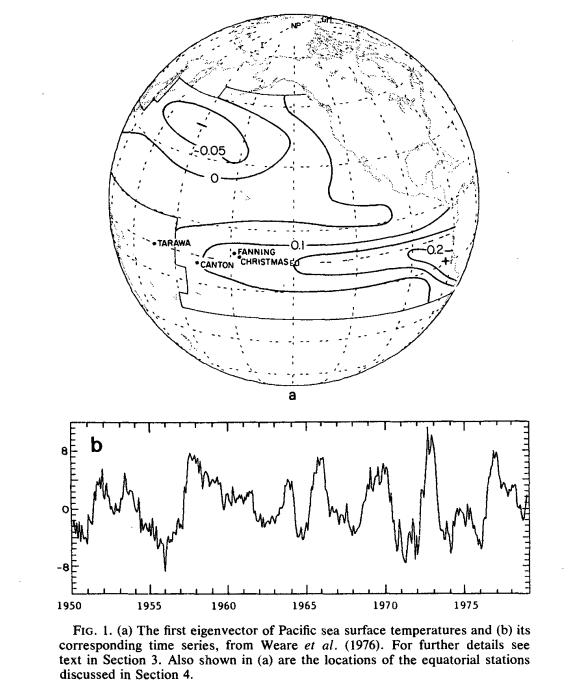
\includegraphics[width=0.5\linewidth]{uploads/Screenshot 2024-11-15 154321.png}
    \caption{Horel and Wallace (1981)}
    \label{fig:1981}
\end{figure}
This prompt was a systematic view with a month timescale variability: they used EOF to analyze 500 mbar data within a month's variability. Are 4 EOFs appearing during the analysis, the matrix had 45 columns (time series). As shown below, these patterns are a succession of positive and negative signs. In picture 16\% of variance: reconstructing the timeserie using only that mode, the total variance of that mode will be 16\% of the variance, or, having 45 modes, construct one by change, the change that it will look close to that one is 16\%.
\begin{figure}[h!]
    \centering
    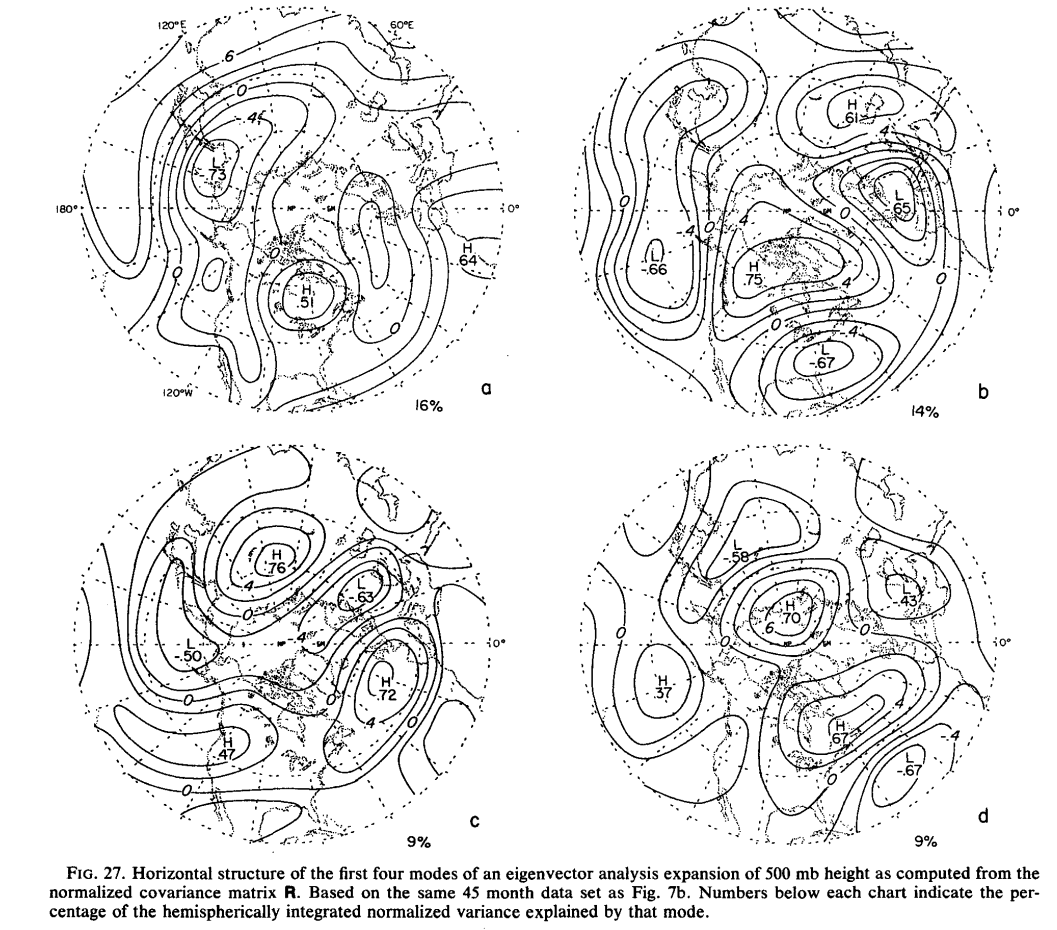
\includegraphics[width=0.5\linewidth]{uploads/Screenshot 2024-11-15 155150.png}
    \caption{Correlation coefficients}
    \label{fig:correlation coeff}
\end{figure}
There was a network of connections disappearing beyond the synoptic view, beyond monthly timescales there's a network of connections. Synoptic variation was understood as an instability of the basic flow. You will reach a nonlinear balance if the instability grows very much outside the linear regime, and this could happen in a time series of a week/ten days. 
When you try to connect variability in the ocean with the variability in the atmosphere you get a pattern like the one below (slide 15).

The idea came forward that at least a part of this teleconnection must be connected to the Ocean. There's a lot of variability in the ocean at monthly timescales. The figure below \ref{fig:SST VAR} shows deviations from seasonal timescales: a lot of variability at monthly timescales. The figure also shows the strongest El Nino ever recorded in 1993 and in 1998 another El Nino.
\begin{figure}[h!]
    \centering
    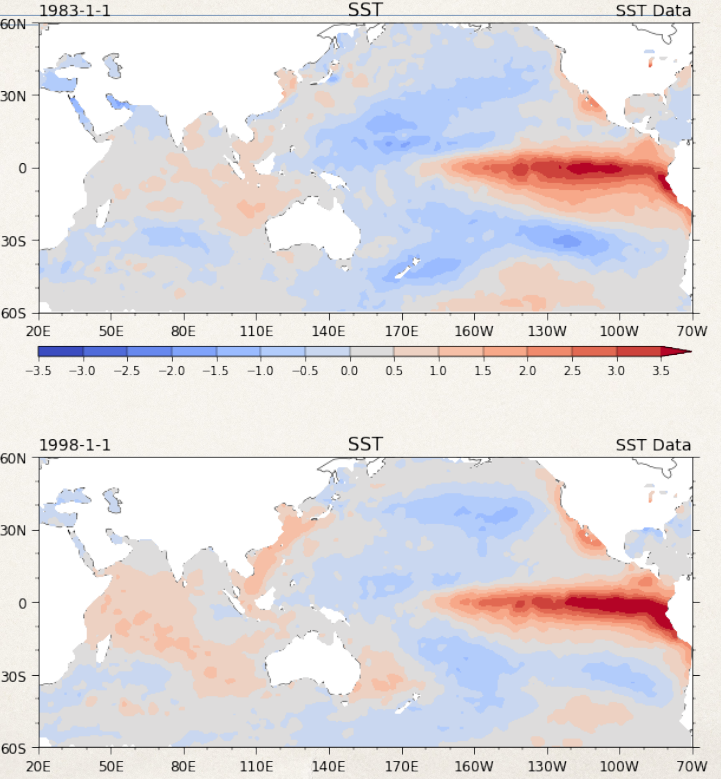
\includegraphics[width=0.5\linewidth]{uploads/Screenshot 2024-11-18 164612.png}
    \caption{SST Variability over a monthly timescale}
    \label{fig:SST VAR}
\end{figure}

\begin{figure}[h!]
    \centering
    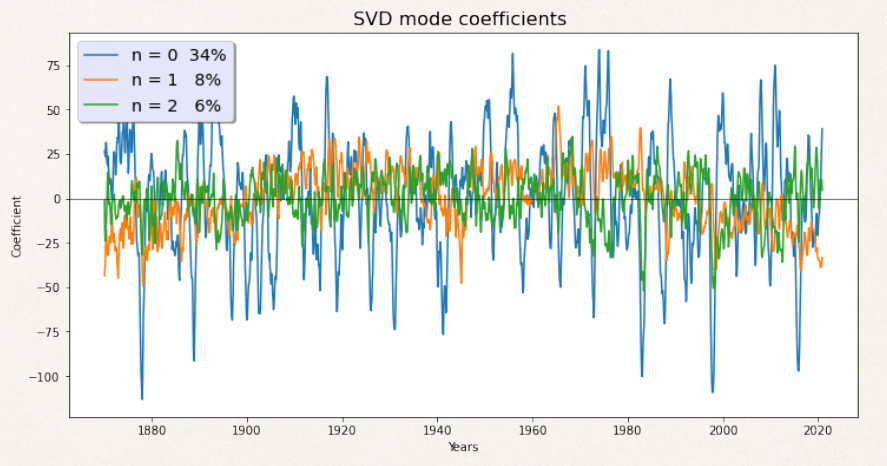
\includegraphics[width=0.5\linewidth]{uploads/Screenshot 2024-11-18 164205.png}
    \caption{Main EOF time series}
    \label{fig:eof time series}
\end{figure}
Figure \ref{fig:eof time series} represents a modern analysis of SST variability from 1880 to last year. Once the notion that the SST was important, became clear, people started to try to record the SST. However, there could have been a problem due to the difference in heat loss between different stations. In the figure, $n=0$ is the first EOF, here you can see huge oscillations (describes ENSO) and the negative phases of ENSO that are oscillating down. From now on started to come out with the idea that there is some periodic behavior. 
\begin{figure}[h!]
    \centering
    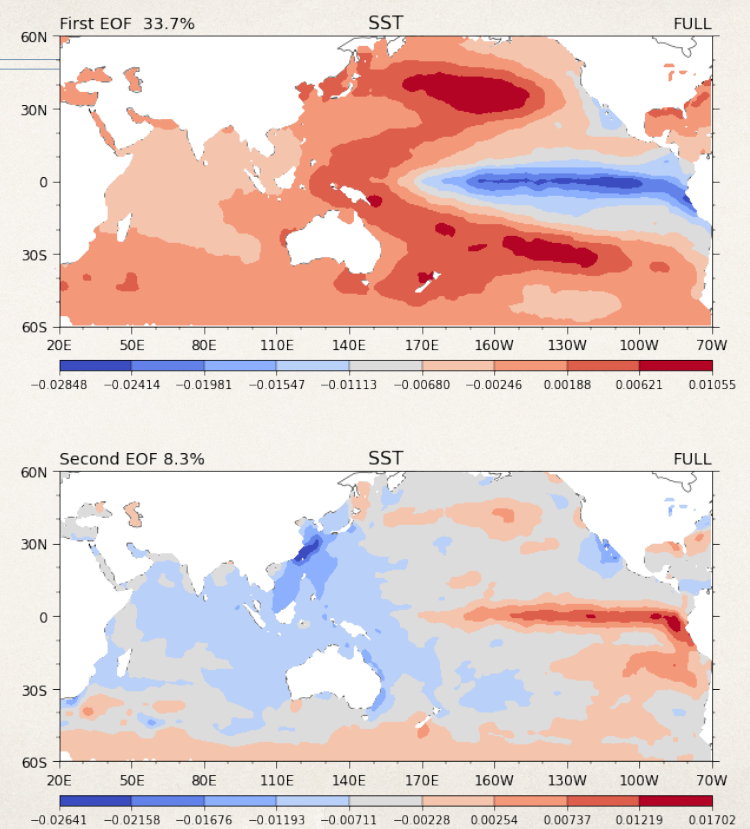
\includegraphics[width=0.5\linewidth]{uploads/Screenshot 2024-11-18 164916.png}
    \caption{First two modes}
    \label{fig:first two modes}
\end{figure}
In figure \ref{fig:first two modes}: the top one of El Nino, EOF cannot separate one phenomenon from the other: there are mathematical constraints (i.e. to be orthogonal to each other). In the following  years, people try to make variations to address some of the problems. EOFs are very sensitive to where the variability is concentrated. As you go to higher modes, you get more structure for two main reasons: modes are getting more complicated and EOFs have to be orthogonal to each other because of their construction. Everything is dominated by the large variations in the equatorial zone, and this variation in the North Pacific is relatively weighted less (here is very uniform but something is going on). Later it was discovered to be the Pacific decayed oscillation. 

All of these evidences were statistics, there is no reason to believe in causation. In order to demonstrate that is the SST creating those oscillations, use a climate model: you have to design an experiment. I have evidence from experiments that SST is connected to the anomaly in the atmosphere, what should I do? I need to design a numerical, that is a  simulation of climate using the model. 
For instance, we would like to see the evolution in time of SST and we have a dataset from 1880. 
Considering just the atmosphere, you need initial data in the model and boundary conditions in the ground (topography stressing the presence of mountains, it is not necessary to consider vegetation because it is part of the length scheme of the model, but we need a land-see mask stressing where are lands, oceans and ice). You have to take into account the temperature of the ocean, in this case, SST (integrating forward in time will get a simulation in data). If you want to see the impact of the SST on the atmosphere you change the model inducing a disturbance (for example, changing the boundary conditions at the surface) and you get the monthly mean of SST. This type of experiment is called a prescribed experiment.

run an atm model where we see the mean SST for the entire simulation of the model (temperature at 2 m is part of the atm problem). artificially increasing --> putting a perturbation in some areas slide 21.  ????

So they built a strategy to do that: you start with a basic model and you add a perturbation to it. This will lead you to a comparison between one system with the perturbation and the other one without the perturbation, which is called the control system or the reference. Comparing the two systems I obtained, I'll gain the effect of the perturbation I applied. 

\begin{figure}
    \centering
    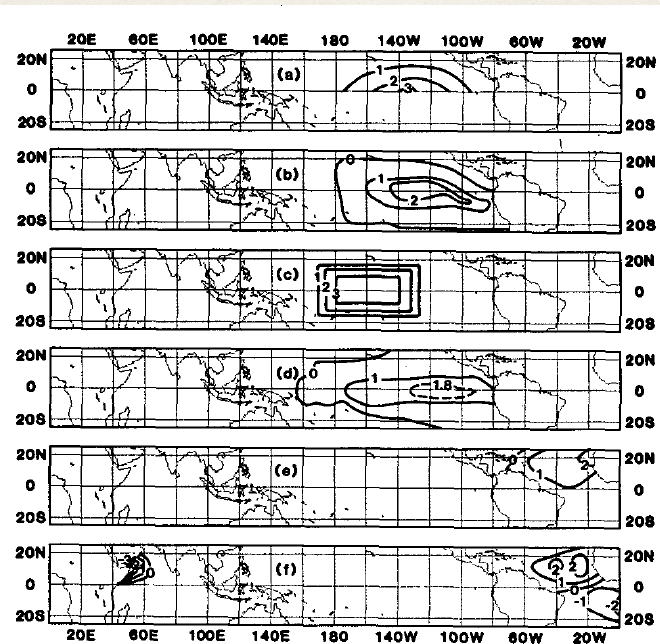
\includegraphics[width=0.5\linewidth]{uploads/Screenshot 2024-11-20 212353.png}
    \caption{the fourth from the top is the paper}
    \label{fig:enter-label}
\end{figure}
They did two perturbations and looked at the difference: the model would create a series of anomalies propagating. You create anticyclones in the north and the south of the anomaly. This fact provides an intense investigation of how the monthly scale can predict monthly anomalies. We are taking the difference between two strongly nonlinear simulations, so we are stretching the fact that we can still see the difference. 

This means that the relation of the two simulations is quite linear so that the effect of perturbations can be identified. In detail, consider the geopotential at 300 mbar (high atmosphere), it is the streamfunction of the flow. 
\begin{figure}
    \centering
    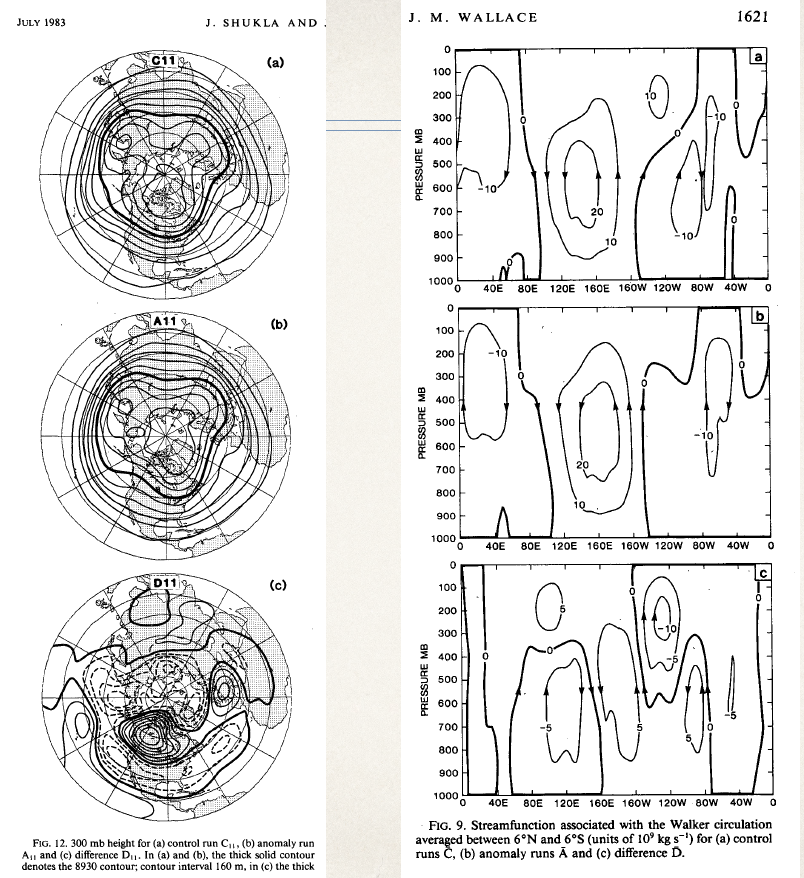
\includegraphics[width=0.5\linewidth]{uploads/Screenshot 2024-11-20 212453.png}
    \caption{Enter Caption}
    \label{fig:enter-label}
\end{figure}
The one on top is the control simulations, the middle one is the perturbation experiment (with SST in the Pacific) and the bottom one is the difference between the two. 
Most of them are concentrated in the North Pacific, related to the SST anomaly in the equatorial Pacific. Note that when you look at the total field the differences are small but still exist.
This was the first evidence that if you have perturbation that will have an impact, that creates a deviation from normal conditions.  

fig 9 is a section at the equator between 6N and 6S 
the arrows give the sense of circulation; in the difference, you see the extra rising air over the SST (central part or graph). This paper shows that the way SST is acting on the atmosphere is affecting the water circulation, especially increasing the vertical motion over the areas of increased SST. Why exactly air go up?

People decided to set up a special project called AMIP, an atmospheric model intercomparison project, based on the idea that SST is important but we have many models, expecting the SST in different ways, so how we could compare them? 
It was already clear that because of the sensitivity not only of the initial conditions but also to perturbation, it is not enough one simulation. 
We know that if we change a little bit initial conditions in any of these models, the evolution is slightly different, and also the response of SST it is; meaning that you have to do different experiments and confront them statistically. 

They aren't using idealizing perturbation of the SST but the observed SST month by month. So it was designed a protocol in which all the people participating in the project, could run the models using the same dataset.  
\begin{figure}
    \centering
    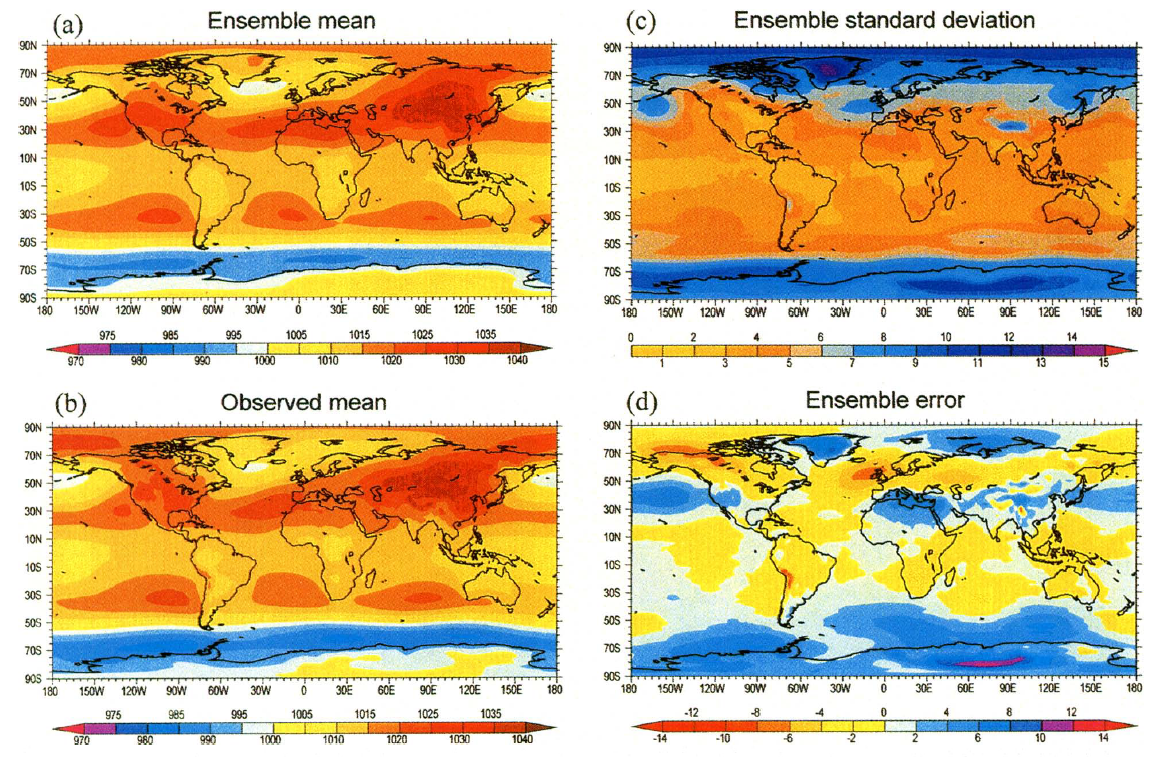
\includegraphics[width=0.5\linewidth]{uploads/Screenshot 2024-11-20 212548.png}
    \caption{AMIP results for mean sea level pressure}
    \label{fig:enter-label}
\end{figure}
As for the mean sea level pressure measured in winter between 1979 and 1988, despite the fact the ensemble means and the observed mean seem to be similar, there is an error of 14 mbar (good or bad depends on what you have to do).
It was clear that there was a systematic problem: models seem to underestimate sea level pressure. If the error had a systematic structure, it could be possible that numerics weren't represented well. 
If we look at the standard deviation of the ensemble, we are looking at how these models would agree with each other (most of the deviation is presented in polar regions). In other words, we are looking at the degree of control that SST exerts on the atmosphere. If the control is perfect, all the models will give the same evolution; if not, models have the freedom to do slightly different things.   
The SST control is very effective in the tropical regions and in the mid-latitudes (east basin of the ocean). Weaker error occurs over North America, so SST seems capable of controlling the anomaly of circulation over it and the tropics; it seems not to have control over Europe (blob of high standard deviation).  

Internal variation (for example, what will happen at 15 o'clock next month) beyond the range of initial conditions cannot be predicted.

\begin{figure}
    \centering
    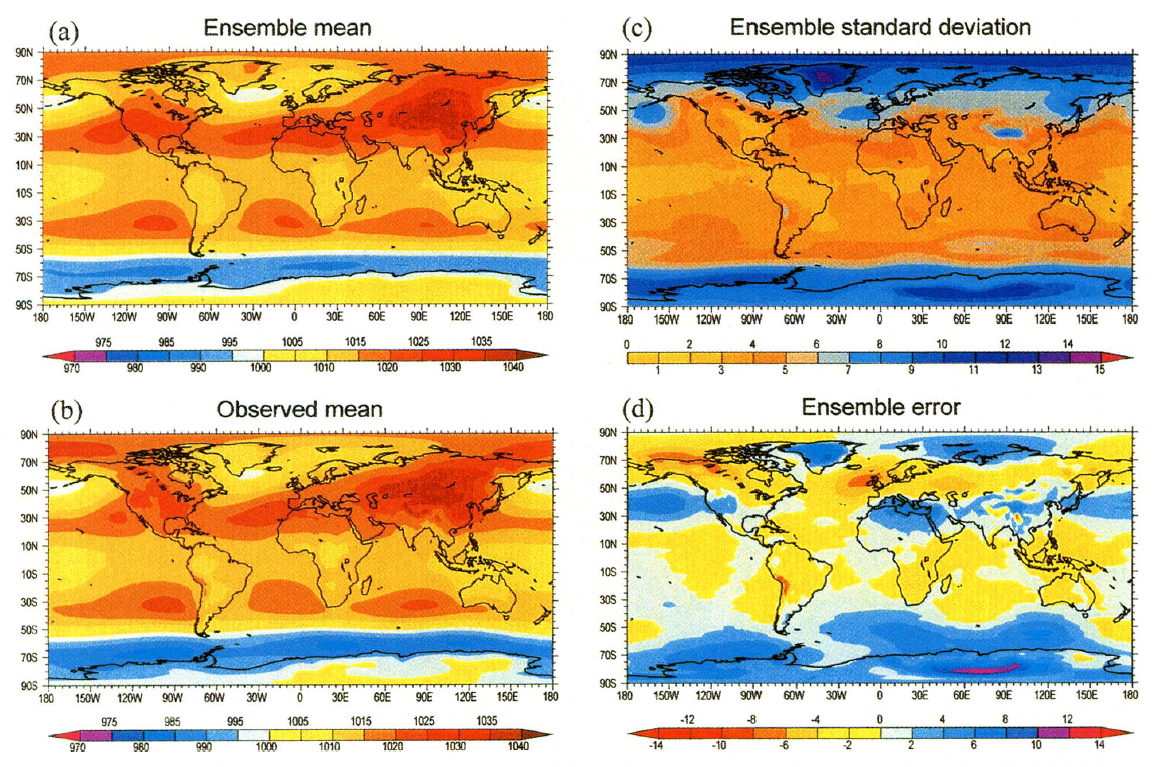
\includegraphics[width=0.5\linewidth]{uploads/Screenshot 2024-11-20 204551.png}
    \caption{AMIP result for precipitations }
    \label{fig:enter-label}
\end{figure}


The standard deviation is very small over the ocean, meaning the SST is controlling precipitations. 
In general, it's much more difficult than the dynamical field, because precipitations are much more difficult than other dynamics since they are driven by physical processes so you need to describe convection and turbulence very well. Other problems are linked with getting the observation and spatial correlation that is difficult. We get good data only recently, especially thanks to satellite like TRIMM that allow us to make estimates of precipitation also over the ocean. 


\begin{figure}
    \centering
    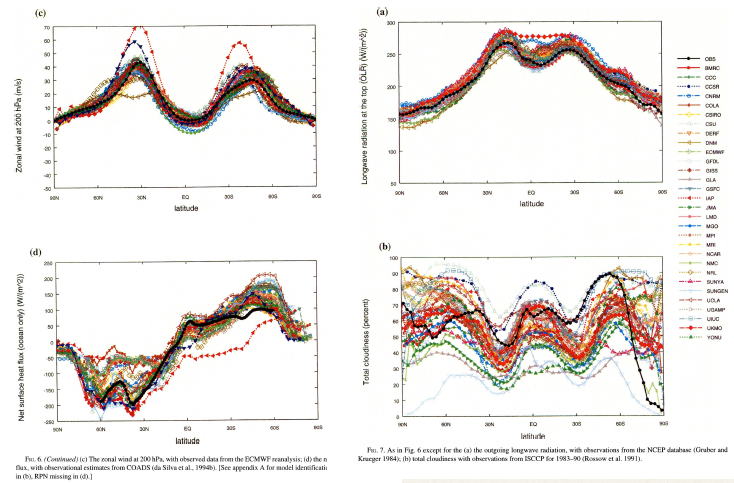
\includegraphics[width=0.5\linewidth]{uploads/Screenshot 2024-11-20 210633.png}
    \caption{all the models participating in the comparison and the observations are the black line}
    \label{fig:enter-label}
\end{figure}
All the models agree on the zonal wind, it means that the dynamics of zonal wind is easy. All the variations you see are how the model is formulated, you start to see differences because different formulation has a big impact, so how people choose to represent them has an impact on the result. 
If your balance at the top is not zero the model will cool or warm over 200-300 years 

(b) disaster. clouds. that shows clouds are difficult. ??


This kind of result grew in people's determination to insert clouds in models because do not consider them to represent the issue of credibility. 



\subsection{General circulation model }
it takes 5-6 years to take experiments that have valid results. 100 years--> climate simulation. what about six months? a climate ex is an experiment in which you try to get equilibrium in external forces (radiation longer timescales, ocean in shorter), once you consider couple modles you have 2 initial conditions: the timescale of their influences is different: the initial conditions of the ocean stay there for a couple of months between 12-15 months. using realistic. seasonal scale: as long as you have initial conditions you get influence, in longer timescales you need a third external source: greenhouse? determine the initial condition has been one of the most seached topics. satelliting sounding in situ stations. you can see that data do not cover uniformally the planet: not homogeneous, they all concentrate in europe. What is the optimal consentration of stations? maximum information with minimum distribution. the problem is that the decision process is almost never dictated by scientific reasons. 
Ocean has been a blackhole for a long time. --> oscean observing system. the green dots are chain of intrument measuring temperature and currents at various steps known as TAO. these are captureted in the area od ENDSO--> sistematic capture of observation. the other things are ARGO floats: instruments bouyands at specific depths. every 10 days they change bouyancy and go up measuring temperature, going to another position. 
these data that you have must be filled in both space and time. I have to find some estimates on the given time in the given area: first thing you can interpolate and fill in the between. the equations are statements of everything you know of the atmosphere: can we use them all to interpolate? --> data simulation is the generic name for this process of estimating space.time evo of the evolution in spacetime of atm and ocean states. the idea is that i'll have physically consistent things. You'll try to minimize the weights of estimation and observations. data simulations sistems allow us to have data on the atm, they are used for forecasting.
re-analysis: comparing all the data sets in the past 50 years with a single ?? we now have hourly data starting from 1949 until today.  use the info you have to modify the model--> data simulation, you then can use this "new state" as the initial condition for a new simulation. step by step you get a sequence of best estimate states of data simulation. both the model and the data simulation tecnique will change over the years . 2024 cannot be compared on an analysis done on 2010. because of the cut i didn't use all the info arrived after the cut (from satellites), we do the simulation without changing system or model--> re-analysis like ERA5. 

\subsection{Ocean transport}
another property that is essential for climate sim but is not a conserved property, is how transport. climate is in part restoring balance in tropics and pole regions. there is an excess rad energy in the equatorial region and a deficit in the polar region. the tropics receive more energy than what they receive. that is ocena transport, done by the atmosphere but the ocean distributes it. 


slide 15 different curves are different ocean re-analysis. black lines are observations. 
in the simulation model slide 16. the observations are the point above, all the lines are model simulations. all the models are underestimating transports. you can manipulate dissipation, turbolence, parameters you can control. you try to optimize the distance between model and observations. 


AMOC circulation in the meridional. it is a part of the global circ of the ocean that starts with the deep water in the Antartica. 2 places where water goes in North atlantic and ?? the hole is closed at the top by surface circulation. in the depth the water goes down. if you stop the production (by freshening the North Atlantic --> increase precipitation), the water will be denser without going down, the transport of heat will "stop". 


slide 22, the plot1 shows the days in which the forecast stopped being useful. in 2020 we reache 7 day--> deterministic limit was pushed from day 5-day 7. this was for deterministic forecast. an ensamble approach. plot2 probabilistic statements beyond that day. deterministic forecast will be with no grey area, prob forecast is more statistical. more observation and then stat analysis. satellite date are measuting emitted radiation transformed in temperature. this t data was ingjected in the data simulation--> massive improvement. our systems are not efficient enough to treat the analysis of everyday. 

errors. I can improve the initial conditions and the model. as the model goes on the error that matter is in the model, iproving the model you improve the medium mode, improving the initial condition you improve short timescale forecast. slide 25 this is the kind of variability you get, some forecasts are completly different: this is the idea of probabilistic forecasts, you take and ensamble and mix statistics with dynamical systems theory. 


%slides 20: atmospheric numerical models

As for the atmospheric models wind, temperature, and water vapor are prognostic variables because they are under time derivative (left part of the equation of motion). Radiation instead, is computed from these variables so it is called a diagnostic variable.
Instead for ocean models, the prognostic ones are currents, temperature, and salinity. The only way to change temperature and salinity is with the interaction between the atmosphere and the ocean. 
Independently from which numerical methods, finite differencing or spectral, we use, we need grids. 
\begin{figure}
    \centering
    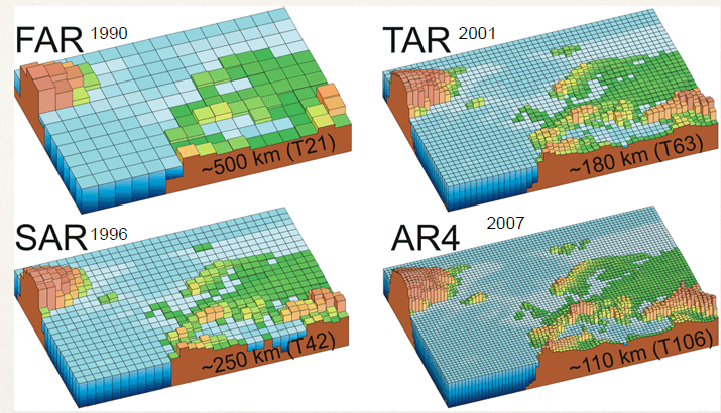
\includegraphics[width=0.5\linewidth]{uploads/Screenshot 2024-11-20 213227.png}
    \caption{Evolution of different models}
    \label{fig:enter-label}
\end{figure}
As we can see from the picture above, FAR had a resolution of 500 km for finite differencing and T21 for the spectral method. Now instead we are able to reach a resolution of 30km x 30km and doing that made us capable of starting to detail the oceans. 